% Options for packages loaded elsewhere
\PassOptionsToPackage{unicode}{hyperref}
\PassOptionsToPackage{hyphens}{url}
%
\documentclass[
]{article}
\usepackage{lmodern}
\usepackage{amssymb,amsmath}
\usepackage{ifxetex,ifluatex}
\ifnum 0\ifxetex 1\fi\ifluatex 1\fi=0 % if pdftex
  \usepackage[T1]{fontenc}
  \usepackage[utf8]{inputenc}
  \usepackage{textcomp} % provide euro and other symbols
\else % if luatex or xetex
  \usepackage{unicode-math}
  \defaultfontfeatures{Scale=MatchLowercase}
  \defaultfontfeatures[\rmfamily]{Ligatures=TeX,Scale=1}
\fi
% Use upquote if available, for straight quotes in verbatim environments
\IfFileExists{upquote.sty}{\usepackage{upquote}}{}
\IfFileExists{microtype.sty}{% use microtype if available
  \usepackage[]{microtype}
  \UseMicrotypeSet[protrusion]{basicmath} % disable protrusion for tt fonts
}{}
\makeatletter
\@ifundefined{KOMAClassName}{% if non-KOMA class
  \IfFileExists{parskip.sty}{%
    \usepackage{parskip}
  }{% else
    \setlength{\parindent}{0pt}
    \setlength{\parskip}{6pt plus 2pt minus 1pt}}
}{% if KOMA class
  \KOMAoptions{parskip=half}}
\makeatother
\usepackage{xcolor}
\IfFileExists{xurl.sty}{\usepackage{xurl}}{} % add URL line breaks if available
\IfFileExists{bookmark.sty}{\usepackage{bookmark}}{\usepackage{hyperref}}
\hypersetup{
  pdftitle={Statistical Inference Course Project Part 2},
  pdfauthor={Pulan Yu},
  hidelinks,
  pdfcreator={LaTeX via pandoc}}
\urlstyle{same} % disable monospaced font for URLs
\usepackage[margin=1in]{geometry}
\usepackage{color}
\usepackage{fancyvrb}
\newcommand{\VerbBar}{|}
\newcommand{\VERB}{\Verb[commandchars=\\\{\}]}
\DefineVerbatimEnvironment{Highlighting}{Verbatim}{commandchars=\\\{\}}
% Add ',fontsize=\small' for more characters per line
\usepackage{framed}
\definecolor{shadecolor}{RGB}{248,248,248}
\newenvironment{Shaded}{\begin{snugshade}}{\end{snugshade}}
\newcommand{\AlertTok}[1]{\textcolor[rgb]{0.94,0.16,0.16}{#1}}
\newcommand{\AnnotationTok}[1]{\textcolor[rgb]{0.56,0.35,0.01}{\textbf{\textit{#1}}}}
\newcommand{\AttributeTok}[1]{\textcolor[rgb]{0.77,0.63,0.00}{#1}}
\newcommand{\BaseNTok}[1]{\textcolor[rgb]{0.00,0.00,0.81}{#1}}
\newcommand{\BuiltInTok}[1]{#1}
\newcommand{\CharTok}[1]{\textcolor[rgb]{0.31,0.60,0.02}{#1}}
\newcommand{\CommentTok}[1]{\textcolor[rgb]{0.56,0.35,0.01}{\textit{#1}}}
\newcommand{\CommentVarTok}[1]{\textcolor[rgb]{0.56,0.35,0.01}{\textbf{\textit{#1}}}}
\newcommand{\ConstantTok}[1]{\textcolor[rgb]{0.00,0.00,0.00}{#1}}
\newcommand{\ControlFlowTok}[1]{\textcolor[rgb]{0.13,0.29,0.53}{\textbf{#1}}}
\newcommand{\DataTypeTok}[1]{\textcolor[rgb]{0.13,0.29,0.53}{#1}}
\newcommand{\DecValTok}[1]{\textcolor[rgb]{0.00,0.00,0.81}{#1}}
\newcommand{\DocumentationTok}[1]{\textcolor[rgb]{0.56,0.35,0.01}{\textbf{\textit{#1}}}}
\newcommand{\ErrorTok}[1]{\textcolor[rgb]{0.64,0.00,0.00}{\textbf{#1}}}
\newcommand{\ExtensionTok}[1]{#1}
\newcommand{\FloatTok}[1]{\textcolor[rgb]{0.00,0.00,0.81}{#1}}
\newcommand{\FunctionTok}[1]{\textcolor[rgb]{0.00,0.00,0.00}{#1}}
\newcommand{\ImportTok}[1]{#1}
\newcommand{\InformationTok}[1]{\textcolor[rgb]{0.56,0.35,0.01}{\textbf{\textit{#1}}}}
\newcommand{\KeywordTok}[1]{\textcolor[rgb]{0.13,0.29,0.53}{\textbf{#1}}}
\newcommand{\NormalTok}[1]{#1}
\newcommand{\OperatorTok}[1]{\textcolor[rgb]{0.81,0.36,0.00}{\textbf{#1}}}
\newcommand{\OtherTok}[1]{\textcolor[rgb]{0.56,0.35,0.01}{#1}}
\newcommand{\PreprocessorTok}[1]{\textcolor[rgb]{0.56,0.35,0.01}{\textit{#1}}}
\newcommand{\RegionMarkerTok}[1]{#1}
\newcommand{\SpecialCharTok}[1]{\textcolor[rgb]{0.00,0.00,0.00}{#1}}
\newcommand{\SpecialStringTok}[1]{\textcolor[rgb]{0.31,0.60,0.02}{#1}}
\newcommand{\StringTok}[1]{\textcolor[rgb]{0.31,0.60,0.02}{#1}}
\newcommand{\VariableTok}[1]{\textcolor[rgb]{0.00,0.00,0.00}{#1}}
\newcommand{\VerbatimStringTok}[1]{\textcolor[rgb]{0.31,0.60,0.02}{#1}}
\newcommand{\WarningTok}[1]{\textcolor[rgb]{0.56,0.35,0.01}{\textbf{\textit{#1}}}}
\usepackage{graphicx,grffile}
\makeatletter
\def\maxwidth{\ifdim\Gin@nat@width>\linewidth\linewidth\else\Gin@nat@width\fi}
\def\maxheight{\ifdim\Gin@nat@height>\textheight\textheight\else\Gin@nat@height\fi}
\makeatother
% Scale images if necessary, so that they will not overflow the page
% margins by default, and it is still possible to overwrite the defaults
% using explicit options in \includegraphics[width, height, ...]{}
\setkeys{Gin}{width=\maxwidth,height=\maxheight,keepaspectratio}
% Set default figure placement to htbp
\makeatletter
\def\fps@figure{htbp}
\makeatother
\setlength{\emergencystretch}{3em} % prevent overfull lines
\providecommand{\tightlist}{%
  \setlength{\itemsep}{0pt}\setlength{\parskip}{0pt}}
\setcounter{secnumdepth}{-\maxdimen} % remove section numbering

\title{Statistical Inference Course Project Part 2}
\author{Pulan Yu}
\date{2/29/2020}

\begin{document}
\maketitle

\hypertarget{part-2-basic-inferential-data-analysis}{%
\subsection{Part 2: Basic Inferential Data
Analysis}\label{part-2-basic-inferential-data-analysis}}

ToothGrowth dataset has three columns: len, supp and dos. The supp is a
factor with two levels: VC and OJ. The dose has three values: 0.5, 1.0
and 2.0. The following code will do an exploeratory analysis

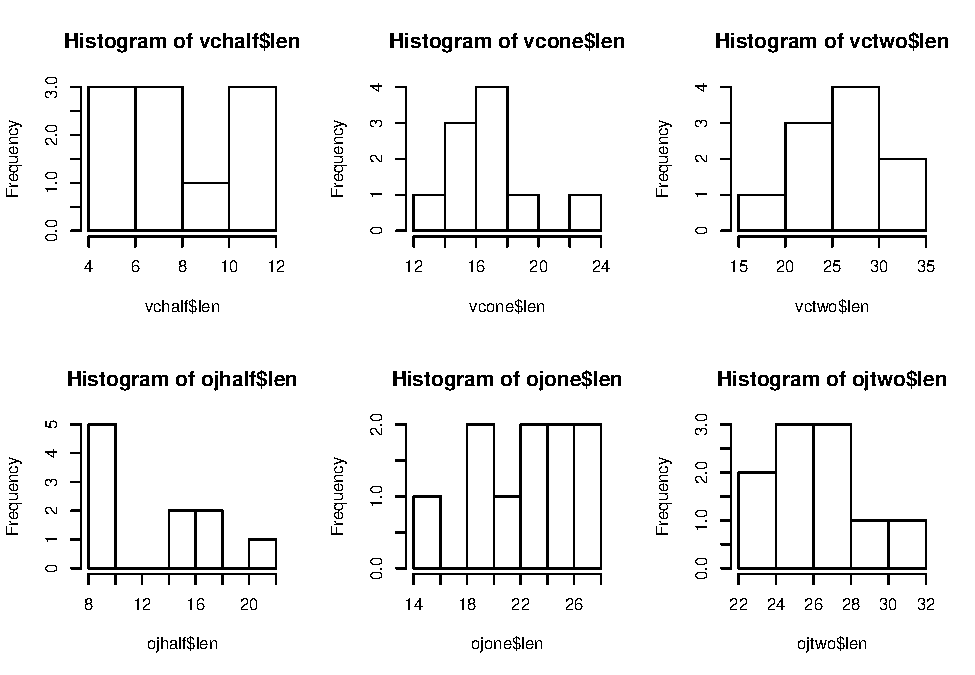
\includegraphics{Final_project_2_final_files/figure-latex/unnamed-chunk-1-1.pdf}

Supp has two values: VC and OJ respectively. The dose has five levels
from 0.5,1.0,to 2.0.

\begin{Shaded}
\begin{Highlighting}[]
  \KeywordTok{par}\NormalTok{(}\DataTypeTok{mfrow=}\KeywordTok{c}\NormalTok{(}\DecValTok{1}\NormalTok{,}\DecValTok{2}\NormalTok{))}
\NormalTok{  vc <-}\StringTok{ }\NormalTok{ToothGrowth[ToothGrowth}\OperatorTok{$}\NormalTok{supp }\OperatorTok{==}\StringTok{'VC'}\NormalTok{,]}
  \KeywordTok{boxplot}\NormalTok{(vc}\OperatorTok{$}\NormalTok{len}\OperatorTok{~}\NormalTok{vc}\OperatorTok{$}\NormalTok{dos,}\DataTypeTok{col=}\NormalTok{(}\KeywordTok{c}\NormalTok{(}\StringTok{"red"}\NormalTok{,}\StringTok{"gold"}\NormalTok{,}\StringTok{"darkgreen"}\NormalTok{)),}\DataTypeTok{xlab =} \StringTok{'dos'}\NormalTok{,}\DataTypeTok{ylab=}\StringTok{'len'}\NormalTok{,}\DataTypeTok{main=}\StringTok{"VC"}\NormalTok{)}
\NormalTok{  oj <-}\StringTok{ }\NormalTok{ToothGrowth[ToothGrowth}\OperatorTok{$}\NormalTok{supp }\OperatorTok{==}\StringTok{'OJ'}\NormalTok{,]}
  \KeywordTok{boxplot}\NormalTok{(oj}\OperatorTok{$}\NormalTok{len}\OperatorTok{~}\NormalTok{oj}\OperatorTok{$}\NormalTok{dos,}\DataTypeTok{col=}\NormalTok{(}\KeywordTok{c}\NormalTok{(}\StringTok{"red"}\NormalTok{,}\StringTok{"gold"}\NormalTok{,}\StringTok{"darkgreen"}\NormalTok{)),}\DataTypeTok{xlab=}\StringTok{'dos'}\NormalTok{,}\DataTypeTok{ylab=}\StringTok{'len'}\NormalTok{,}\DataTypeTok{main=}\StringTok{'OJ'}\NormalTok{)}
\end{Highlighting}
\end{Shaded}

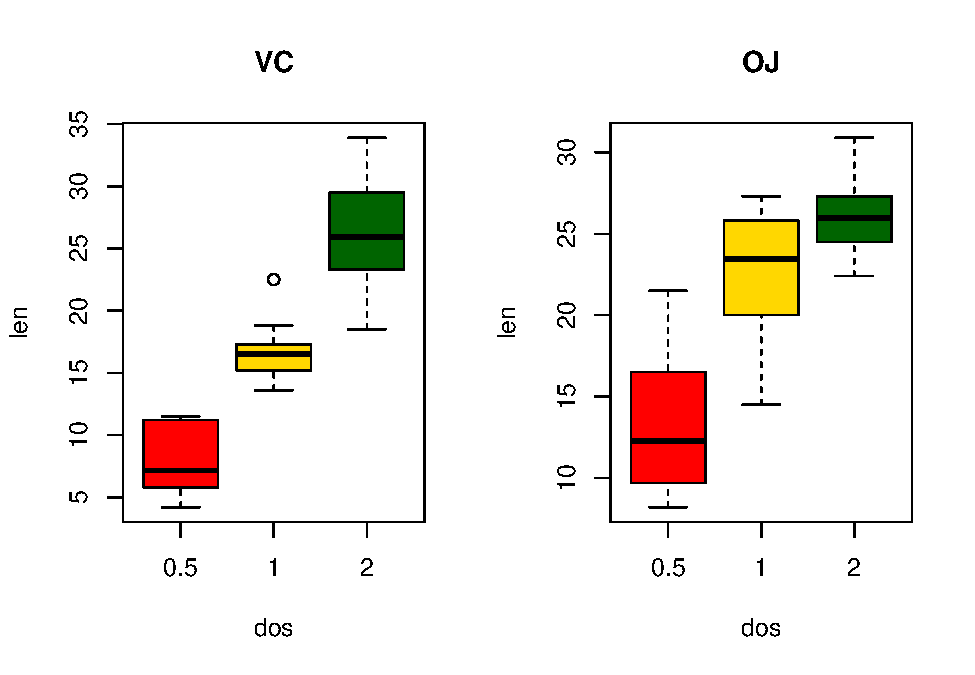
\includegraphics{Final_project_2_final_files/figure-latex/unnamed-chunk-2-1.pdf}

Since there are two variables: supp and dose, firstly, the effect of
dose is investigated. The result format is confidence interval followed
by P-Value

\begin{enumerate}
\def\labelenumi{\arabic{enumi}.}
\tightlist
\item
  the 0.5 level
\end{enumerate}

\begin{Shaded}
\begin{Highlighting}[]
\NormalTok{  vchalf <-}\StringTok{ }\NormalTok{vc[vc}\OperatorTok{$}\NormalTok{dose}\OperatorTok{==}\FloatTok{0.5}\NormalTok{,]}
\NormalTok{  ojhalf <-}\StringTok{ }\NormalTok{oj[oj}\OperatorTok{$}\NormalTok{dose}\OperatorTok{==}\FloatTok{0.5}\NormalTok{,]}
\NormalTok{  test <-}\StringTok{ }\KeywordTok{t.test}\NormalTok{(vchalf}\OperatorTok{$}\NormalTok{len,ojhalf}\OperatorTok{$}\NormalTok{len,}\DataTypeTok{var.equal=}\OtherTok{TRUE}\NormalTok{)}
\NormalTok{  res <-}\StringTok{ }\KeywordTok{c}\NormalTok{(test}\OperatorTok{$}\NormalTok{conf.int,test}\OperatorTok{$}\NormalTok{p.value)}
  \KeywordTok{print}\NormalTok{(res)}
\end{Highlighting}
\end{Shaded}

\begin{verbatim}
## [1] -8.729738345 -1.770261655  0.005303661
\end{verbatim}

\begin{enumerate}
\def\labelenumi{\arabic{enumi}.}
\setcounter{enumi}{1}
\tightlist
\item
  the 1.0 level
\end{enumerate}

\begin{verbatim}
## [1] -9.0193080513 -2.8406919487  0.0007807262
\end{verbatim}

\begin{enumerate}
\def\labelenumi{\arabic{enumi}.}
\setcounter{enumi}{2}
\tightlist
\item
  the 2.0 level
\end{enumerate}

\begin{verbatim}
## [1] -3.5629985  3.7229985  0.9637098
\end{verbatim}

Then the effect of dose is investigated.

For VC supply

\begin{Shaded}
\begin{Highlighting}[]
\NormalTok{  vchalf <-}\StringTok{ }\NormalTok{vc[vc}\OperatorTok{$}\NormalTok{dose}\OperatorTok{==}\FloatTok{0.5}\NormalTok{,]}
\NormalTok{  vcone <-}\StringTok{ }\NormalTok{vc[vc}\OperatorTok{$}\NormalTok{dose}\OperatorTok{==}\FloatTok{1.0}\NormalTok{,]}
\NormalTok{  vctwo <-}\StringTok{ }\NormalTok{vc[vc}\OperatorTok{$}\NormalTok{dose}\OperatorTok{==}\FloatTok{2.0}\NormalTok{,]}
\NormalTok{  test <-}\StringTok{ }\KeywordTok{t.test}\NormalTok{(vchalf}\OperatorTok{$}\NormalTok{len,vcone}\OperatorTok{$}\NormalTok{len,}\DataTypeTok{var.equal=}\OtherTok{TRUE}\NormalTok{)}
\NormalTok{  res <-}\StringTok{ }\KeywordTok{c}\NormalTok{(test}\OperatorTok{$}\NormalTok{conf.int,test}\OperatorTok{$}\NormalTok{p.value)}
  \KeywordTok{print}\NormalTok{(}\StringTok{'Dose 0.5'}\NormalTok{)}
\end{Highlighting}
\end{Shaded}

\begin{verbatim}
## [1] "Dose 0.5"
\end{verbatim}

\begin{Shaded}
\begin{Highlighting}[]
  \KeywordTok{print}\NormalTok{(res)}
\end{Highlighting}
\end{Shaded}

\begin{verbatim}
## [1] -1.126435e+01 -6.315654e+00  6.492265e-07
\end{verbatim}

\begin{Shaded}
\begin{Highlighting}[]
\NormalTok{  test <-}\StringTok{ }\KeywordTok{t.test}\NormalTok{(vchalf}\OperatorTok{$}\NormalTok{len,vctwo}\OperatorTok{$}\NormalTok{len,}\DataTypeTok{var.equal=}\OtherTok{TRUE}\NormalTok{)}
\NormalTok{  res <-}\StringTok{ }\KeywordTok{c}\NormalTok{(test}\OperatorTok{$}\NormalTok{conf.int,test}\OperatorTok{$}\NormalTok{p.value)}
  \KeywordTok{print}\NormalTok{(}\StringTok{'Dose 1.0'}\NormalTok{)}
\end{Highlighting}
\end{Shaded}

\begin{verbatim}
## [1] "Dose 1.0"
\end{verbatim}

\begin{Shaded}
\begin{Highlighting}[]
  \KeywordTok{print}\NormalTok{(res)}
\end{Highlighting}
\end{Shaded}

\begin{verbatim}
## [1] -2.183284e+01 -1.448716e+01  4.957286e-09
\end{verbatim}

\begin{Shaded}
\begin{Highlighting}[]
\NormalTok{  test <-}\StringTok{ }\KeywordTok{t.test}\NormalTok{(vctwo}\OperatorTok{$}\NormalTok{len,vcone}\OperatorTok{$}\NormalTok{len,}\DataTypeTok{var.equal=}\OtherTok{TRUE}\NormalTok{)}
\NormalTok{  res <-}\StringTok{ }\KeywordTok{c}\NormalTok{(test}\OperatorTok{$}\NormalTok{conf.int,test}\OperatorTok{$}\NormalTok{p.value)}
  \KeywordTok{print}\NormalTok{(}\StringTok{'Dose 2.0'}\NormalTok{)}
\end{Highlighting}
\end{Shaded}

\begin{verbatim}
## [1] "Dose 2.0"
\end{verbatim}

\begin{Shaded}
\begin{Highlighting}[]
  \KeywordTok{print}\NormalTok{(res)}
\end{Highlighting}
\end{Shaded}

\begin{verbatim}
## [1] 5.771040e+00 1.296896e+01 3.397578e-05
\end{verbatim}

For OJ supply

\begin{verbatim}
## [1] "Dose 0.5"
\end{verbatim}

\begin{verbatim}
## [1] -1.341081e+01 -5.529186e+00  8.357559e-05
\end{verbatim}

\begin{verbatim}
## [1] "Dose 1.0"
\end{verbatim}

\begin{verbatim}
## [1] -1.627822e+01 -9.381777e+00  3.401859e-07
\end{verbatim}

\begin{verbatim}
## [1] "Dose 2.0"
\end{verbatim}

\begin{verbatim}
## [1] 0.2194983 6.5005017 0.0373628
\end{verbatim}

Conclusions:

For both OJ and VC supply, the level of difference has effect on the
tooth length since the p-value of all t-test are less then 0.05 at 95\%
confidence level. The null hypothesis is rejected, the level has effect
on the length and higher does is better for tooth growth.

For the same level, at low dose level 0.5 and 1.0, the supply has effect
on the tooth length and OJ is better for tooth growth. Since the p-value
of 0.5 and 1.0 level are 0.005304 and 0.0007807 respectively, so the
null hypothesis is rejected and supply has impact on the length. For 2.0
level, the p-value is 0.9637, the null hypothese is failed to be
rejected at 95\% confidence level. It suggests that at high dose, the
supply may not have statistical significant impact on tooth length.

\end{document}
